\documentclass[12pt, fleqn]{article}
\usepackage[serbian]{babel}

% \usepackage{thesis}
% \newcommand{\thesisName}{Hardverska implementacija Viola-Jones algoritma}

\author{Risto Pejašinović}
\date{}

\usepackage{glossaries}
\usepackage{thesis}
\usepackage{glossary}
\usepackage{amsmath}
\usepackage{bytefield}
\usepackage{register}
% \newcommand{\thesisName}{Hardverska implementacija Viola-Jones algoritma}
% % \newcommand{\subjectName}{Projekat iz predmeta Projektovanje elektronskih uređaja na sistemskom nivou}

% \author{Risto Pejašinović EE19/2015}
% \newcommand{\mentor}{}
% \date{septembar 2019}

% \selectcolormodel{gray}


\usepackage{fancyhdr}
\usepackage{lipsum}% just to generate text for the example
\pagestyle{fancy}
\renewcommand{\headrulewidth}{0.4pt}% Default \headrulewidth is 0.4pt
\fancyhead[L]{}

\begin{document}
%% listing and figure numbering per section %%
\counterwithin{lstlisting}{section}
\counterwithin{figure}{section}
\counterwithin{equation}{section}
\counterwithin{table}{section}
% \titlePageCmd
\pagenumbering{}

% 
\includepdf[pages={0,1},pagecommand={}]{template.pdf}

\includepdf[pages={1,2},pagecommand={}]{template.pdf}
\pagenumbering{arabic}
\setcounter{page}{3}

\includepdf[pages={3,4},pagecommand={}]{template.pdf}
\noindent

% \thispagestyle{empty}
% \newpage

\tableofcontents

\newpage
\listoffigures

\newpage
\listoftables

\lstlistoflistings

\newpage
\newacronym{uvm}{UVM}{Universal Verification Methodology}
\newacronym{sv}{SV}{System Verilog}
\newacronym{tb}{TB}{Testbench}
\newacronym{dut}{DUT}{Design under test}
\newacronym{sc}{SC}{SystemC}
\newacronym{hdl}{HDL}{Hardware Description Language}
\newacronym{hls}{HLS}{High Level Synthesis}
\newacronym{rtl}{RTL}{Register Transfer Methodology}
\newacronym{oop}{OOP}{Object Oriented Programming}
\newacronym{esl}{ESL}{Electronic System Level Design and Verification}
\newacronym{dti}{DTI}{Data Transfer Interface}
\newacronym{so}{SO}{Shared Object}
\newacronym{eda}{EDA}{Electronic Design Automation}
\newacronym{vcd}{VCD}{Value Change Dump}
\newacronym{osh}{OSH}{Open Source Hardware}
\newacronym{spice}{SPICE}{Simulation Program with Integrated Circuit Emphasis}
\newacronym{ode}{ODE}{Ordinary Differential Equation}
\newacronym{ivp}{IVP}{Initial Value Problem}
\newacronym{tlm}{TLM}{Transaction Layer Modeling}
\newacronym{snr}{SNR}{Signal to Noise Ratio}
\newacronym{iir}{IIR}{Infinite Impulse Response}
\newacronym{fir}{FIR}{Finite Impulse Response}
\newacronym{pid}{PID}{Proportional-integral-derivative controller}
\newacronym{blds}{BLDS}{Brushless DC}
\newacronym{smps}{SMPS}{Switching Mode Power Supply}
\newacronym{pwm}{PWM}{Pulse Width Modulation}
\newacronym{gui}{GUI}{Graphical User Interface}

\printglossary[type=\acronymtype,style=mystyle]
\newpage

\section{Viola-Jones algoritam}

\subsection{Uvod}

Namena algoritma je detekcija i lokalizacija objekata na slici. Osmišljen od
strane Paul Viola i Michael Jones 2001. godine \cite{Viola2001RapidOD}.

Dugo godina je zbog brze i pouzdane detekcije bio standardan način detekcije
lica na slici. I danas je prisutan u velikom broju mobilnih telefona i
digitalnih kamera, ali danas postaje polako zamenjen konvolucionim neuronskim
mrežama. \\

Pouzdanost i brzina su postignuti uvođenjem tri ključna doprinosa:
\begin{itemize}

\item \textbf{Integralna slika} omogućava brzo izračunavanje obeležja.
\item \textbf{AdaBoost} algoritam za učenje, odabiranjem obeležja povećava
  brzinu i pouzdanost detekcije.
\item \textbf{Kaskadni klasifikator} Realizovanjem algoritma u kaskadama
  omogućava brzo odbacivanje pozadine slike kako je mala verovatnoća da će se tu
  naći lice. \\
\end{itemize}


\subsection{Integralna slika}

Kao jedan od ključnih delova algoritma, integralna slika omogućava izračunavanje
površine svakog pravougana obeležja u konstantnom vremenu.

Intenzitet piksela u integralnoj slici na poziciji x,y je zbir svih piksela koji
se nalaze gore i levo od pozicije x,y.

\begin{equation}
  \Scale[1.4]{ii(x,y)=\sum\limits_{x'\leq x, y'\leq y} i(x',y')}
  \label{IntegralImage_eq1}
\end{equation}

Gde je ii(x,y) integralna slika, a i(x,y) originalna slika. \\

\begin{figure}[h]
  \centering
  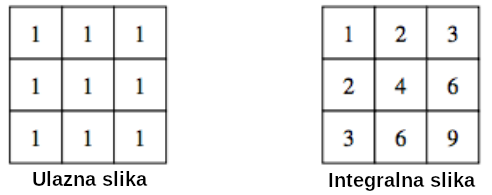
\includegraphics[width=8cm]{integral_image1}
  \caption{Primer integralne slike}
  \label{IntegralImage_img1}
\end{figure}

Piksele integralne slike je moguće računati u paraleli, ili
sekvencijalno. Izbor algoritma za računanje integralne slike značajno utiče na
performanse i potrebne hardverske resurse. \\
U paralelnoj implementaciji cena je
više pristupa memoriji i više potrebnih sabirača, dok je kod sekvencijalne
implementacije manja brzina. \\

Osobina koja integralnu sliku čini pogodnu za korišćenje u Viola-Jones algoritmu
je da je za računanje bilo koje pravougaone površine unutar integralne slike
potrebno 2 sabiranja i 2 oduzimanja.

\begin{figure}[h]
  \centering
  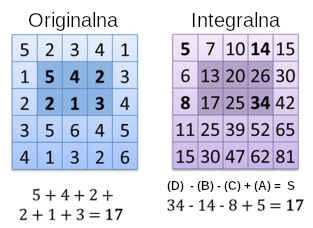
\includegraphics[width=8cm]{integral_image2}
  \caption{Primer računanja površine pravougaonika \cite{IntegralImage1_web}}
  \label{IntegralImage_img2}
\end{figure}

Na slici (\ref{IntegralImage_img2}) je prikazano računanje površine pravougaonika na
originalnoj slici i na integralnoj slici.
Kao što se može videti za površinu pravougaonika MxN na originalnoj slici nam je
potrebno MxN sabiranja. \\
Dok je kod integralne slike broj operacija 2 sabiranja i 2
oduzimanja i ne zavisi od dimenzija pravougaonika.

\begin{equation}
  \Scale[1.4]{\sum\limits_{(x,y)\in ABCD} i(x,y)=ii(D)+ii(A)-ii(B)-ii(C)}
  \cite{Cen2016StudyOV}
  \label{IntegralImage_eq2}
\end{equation}
\newpage

\section{OpenCV modeli} \label{opencv_model}

OpenCV je biblioteka koja sadrži implementacije velikog broja algoritama za
obradu slike.
OpenCV sadrži alat za AdaBoost treniranje kaskadnog klasifikatora kao i implementaciju
detektora objekata pomoću Viola-Jones algoritma. \\
Pored toga OpenCV sadrži istrenirane i testirane modele klasifikatora\footnote{\url{https://github.com/opencv/opencv/tree/master/data/haarcascades}}.
\cite{OpenCV_docs} \\

\noindent
OpenCV istrenirane modele skladišti u .xml fajlove koji sadrže sledeće
informacije o modelu:

\begin{itemize}
	\item Dimenzija obeležja (\emph{height, width})
	\item Broj etapa (\emph{stageNum})
	\item Maksimalan broj obeležja u etapi (\emph{maxWeakCount})
	\item Informacije o etapama (\emph{stages})
    \begin{itemize}
    \item Broj obeležja u etapi (\emph{maxWeakCount})
    \item Prag etape (\emph{stageThreshold})
    \item Informacije o obeležjima (\emph{weakClassifiers})
      \begin{itemize}
      \item Prag obeležja (\emph{internalNodes})
      \item Vrednosti listova (\emph{leafValues})
      \end{itemize}
    \end{itemize}
	\item Informacije o obeležjima (\emph{features})
    \begin{itemize}
    \item Koordinate i težine tačaka pravougaonika (\emph{rects}). \\
      Svako obeležje može imati 2 ili 3 pravougaonika. \\
      Prve 2 vrednosti liste rects su x i y koordinate gornje leve tačke, \\
      treća i četvrta vrednost širina i visina pravougaonika,  \\
      poslednja vrednost je težina pravougaonika.
    \end{itemize}
\end{itemize}

\subsection{OpenCV model za frontalna lica} \label{haarcascade_frontal_sec}

Često korišćeni model za detekciju lica je
\texttt{\detokenize{haarcascade_frontalface_default.xml}}\footnote{\url{https://github.com/opencv/opencv/blob/master/data/haarcascades/haarcascade_frontalface_default.xml}}. \\
Ovaj model se koristi za frontalnu detekciju lica. \\
Neke njegove karakteristike su:
\begin{itemize}
\item Dimenzija obeležja: 24x24
\item Broj etapa: 25
\item Maksimalan broj obeležja u etapi: 211
\item Ukupan broj obeležja: 2913
\end{itemize}

\noindent
Rezultati detekcije ovog modela mogu se videti na
slikama(\ref{sixfaces_scaled},\ref{overexposed_light},\ref{underexposed_light},\ref{rotation_variance},\ref{rotated_res})
iz sekcije \ref{viola_jones_introduction}.
\newpage

\part{Hardverska implementacija}
\section{Sažetak}

Ovaj projekat sadrži:
\begin{itemize}
  \item Projektovanje arhitekture hardverskog akceleratora za Viola-Jones algoritam opisam u delu \ref{viola_jones_algorithm}.
  \item Pisanje specifikacije u Python i C programskom jeziku za izvršavanje i
    pomoć pri particionisanju i projektovanju hardvera.
  \item Pisanje HDL modela za sintezu u SystemVerilog RTL metodologiji i
    \PyGears{} metodologiji.
  \item Pisanje verifikacionog okruženja u SystemVerilog \UVM{} i Python PyGears
    okruženju.
  \item Poređenje dve metodologije i analiza prednosti i mane obe metodologije.
  \item Poređenje komercijalnog \QuestaSim{} simulatora i besplatnog open-source
    \Verilator{} simulatora.
  \item Implementacija projektovanog IP jezgra na \ZTurn{} sa Zynq
    7020 SoC.
  \item Pisanje Linux Kernel drajvera i korisničke aplikacije za korišćenje
    jezgra za detekciju lica na Xilinx Zynq platformi.

\end{itemize}
\newpage
\section{Specifikacije za izršavanje}

Prilikom projektovanja hardverske arhitekture određenog algoritma preporučljivo
je prvo implementirati algoritam u softveru kako bi se algoritam bolje shvatio. \\
Postoje metodologije koje definišu potrebne korake prilikom projektovanja
digitalnih sistema, jedna takva metodologija je \gls{esl}.
U ovom radu nije korišćena ova metodologija već je softverska
specifikacija napisana u C++ i Python jeziku. \\
Iz ovih specifikacija dobijeno je bolje razumevanje algoritma i naznake o
mogućnosti paralelizna određenih delova algoritma i particionisanja komponenti
sistema. \\

\begin{figure}[H]
  \centering
  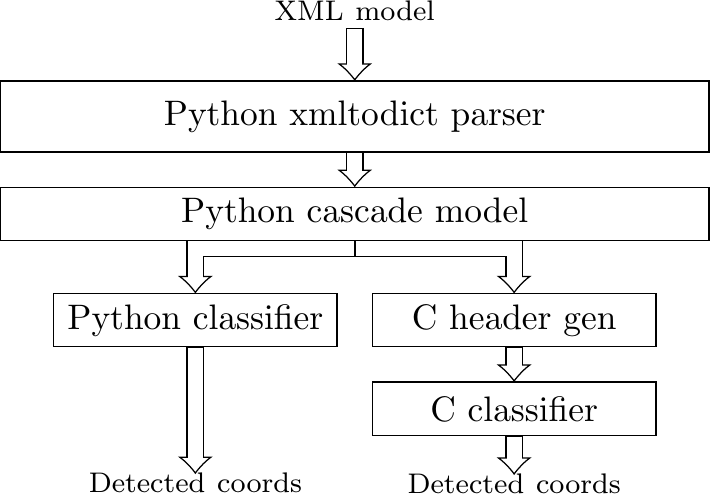
\includegraphics[width=0.9\linewidth]{bdp/sw_arch/sw_arch1.png}
  \caption{Veza Python modela sa XML modelom i C specifikacijom}
  \label{sw_arch_spec1}
\end{figure}

Na slici(\ref{sw_arch_spec1}) prikazana je struktura modela u slučaju Python i C
klasifikatora. \\

\noindent
Na ulazu se nalazi \gls{xml} model dobijen treniranjem pomoću OpenCV biblioteke opisan u sekciji
\ref{opencv_model}. \\
Parsiranje XML modela se rešava u Python-u.
Zbog velikog broja Python paketa dostupnih sa gotovim rešenjima za većinu softverskih problema, problem
parsiranja XML fajla se može rešiti korišćenjem paketa xmltodict\footnote{\url{https://pypi.org/project/xmltodict/}}. \\
\emph{Xmltodict} parsira XML fajl i skladišti ga u Python dictionary. \\
Implementirane su klase \emph{CascadeClass}, \emph{StageClass}, \emph{FeatureClass} i
\emph{RectClass}
\footnote{\texttt{\detokenize{cascade_classifier/python_model/cascade.py}}} koje
predstavljaju abstraktni Python model modela kaskadnog klasifikatora. \\

Napisana je i Python implementacija Viola-Jones algoritma koja koristi Python
model klasifikatora i koristi se kao specifikacija za izvršavanje. \\

Python model klasifikatora može da generiše \emph{C++} reprezentaciju modela
klasifikatora i sačuva ih u Header fajlove. \\
Ovim je izbegnuto parsiranje XML fajlova C++ jezikom, pošto je ovaj zadatak
mnogo jednostavnije odraditi u Python-u. \\
C++ implementacija Viola-Jones algoritma koristi ovako generisan model
klasifikatora.
\newpage
\pgfdeclarelayer{background}
\pgfdeclarelayer{foreground}
\pgfsetlayers{background,main,foreground}

\tikzstyle{cloud1} = [draw=black, thick, fill=red!20, minimum hegiht = 1em]
\tikzstyle{block_l} =[draw, text centered, fill=blue!15, minimum width=3cm, minimum height=3.5cm]
\tikzstyle{block_m} =[draw, text centered, fill=blue!15, minimum width=2.5cm, minimum height=2cm]
\tikzstyle{block_s} =[draw, text centered, fill=blue!15, minimum width=2cm, minimum height=1.5cm]
\tikzstyle{line} = [draw, decoration={markings,mark=at position 1 with {\arrow[scale=2.2,black]{>}}},
    postaction={decorate},
    shorten >=0.4pt]

\begin{tikzpicture}[thick]
  \node [block_l] (img_ram) {IMG RAM};
  \node [coordinate, above = 0cm of img_ram, yshift=-0.5cm, xshift=1.5cm] (img_ram_addr_in){};
  \node [coordinate, left =2.0cm of img_ram] (img_in){};
  \node [coordinate, left = 0cm of img_ram] (img_ram_img_in){};
  \node [coordinate, right = 0cm of img_ram] (img_ram_img_out){};

  \node [block_m, above right = +1cm and 0.2cm of img_ram] (rd_addrgen) {rd\_addrgen};
  \node [coordinate, below = 0cm of rd_addrgen] (rd_addr_addr_out){};

  \node [block_m, above right = -1.75cm and 2.5cm of img_ram ] (ii_gen) {ii\_gen};
  \node [coordinate, left = 0cm of ii_gen] (ii_gen_in){};
  \node [coordinate, right = 0cm of ii_gen] (ii_gen_out){};
  \node [block_m, below = 0.25cm of ii_gen ] (sii_gen) {sii\_gen};
  \node [coordinate, left = 0cm of sii_gen] (sii_gen_in){};
  \node [coordinate, right = 0cm of sii_gen] (sii_gen_out){};

  \node [block_s, right = 1.25cm of sii_gen ] (stddev) {stddev};
  \node [coordinate, above left = -0.25cm and 0cm of stddev] (stddev_ii){};
  \node [coordinate, above left = -0.75cm and 0cm of stddev] (stddev_sii){};
  \node [coordinate, right = 0cm of stddev] (stddev_out){};

  \node [block_m, right = 1.0cm of ii_gen ] (frame_buffer) {frame\_buffer};
  \node [coordinate, left = 0cm of frame_buffer] (frame_buffer_in){};
  \node [coordinate, above left = -0.5cm and 0cm of frame_buffer] (frame_buffer_rect_addr){};
  \node [coordinate, right = 0cm of frame_buffer] (frame_buffer_out){};

  \node [block_m, above = 1.0cm of frame_buffer ] (features_mem) {features\_mem};
  \node [coordinate, left = 0cm of features_mem] (rects_addr){};
  \node [coordinate, right = 0cm of features_mem] (rects_weights){};

  \node [block_l, fill=red!15, above right = -3.5cm and 1cm of frame_buffer] (classifier) {\huge Classifier};
  \node [coordinate, above left = -1cm and 0cm of classifier] (classifier_ii){};
  \node [coordinate, above left = -2.5cm and 0cm of classifier] (classifier_stddev){};
  \node [coordinate, above left = -0.5cm and 0cm of classifier] (classifier_weights){};
  \node [coordinate, above right = -1.0cm and 0cm of classifier] (detected_addr){};
  \node [coordinate, above right = -2.5cm and 0cm of classifier] (irq){};

  %% group %%
 \begin{pgfonlayer}{background}
  \node[inner sep=7pt, fill=yellow!25, rounded corners, inner ysep =30pt, draw, thick,fit=(img_ram) (rd_addrgen) (ii_gen) (features_mem) (sii_gen) (frame_buffer) (stddev) (classifier)] (ip_core) {};
  \node[above left] at (ip_core.south east) {\huge Cascade Classifier IP core};
\end{pgfonlayer}

  % arrows
  \path [line] (rd_addr_addr_out)  |- (img_ram_addr_in) node[transition, xshift=0.8cm, yshift=0.25cm] {rd\_addr};
  \path [line] (img_in) node[transition, yshift=0.25cm, xshift=0.65cm]{\large img\_in} -- (img_ram_img_in);
  \path [line] (img_ram_img_out) node[transition, yshift=0.2cm, xshift=0.9cm] {img\_out} -- +(1.75cm, 0cm) |- (ii_gen_in);
  \path [line] (img_ram_img_out) -- +(1.75cm, 0cm) |- (sii_gen_in);
  \path [line] (ii_gen_out) -- +(0.5cm, 0cm) node[transition, yshift=0.2cm, xshift=0cm] {ii} |- (stddev_ii);
  \path [line] (sii_gen_out) -- +(0.5cm, 0cm)  node[transition, yshift=0.2cm, xshift=0cm] {sii} |- (stddev_sii);
  \path [line] (ii_gen_out) |- (frame_buffer);
  \path [line] (frame_buffer_out) node[transition, yshift=+0.2cm, xshift=0.5cm] {fb\_ii} |- (classifier_ii);
  \path [line] (stddev_out) -- +(0.5cm, 0) node[transition, yshift=-0.2cm, xshift=0.1cm] {stddev} |- (classifier_stddev);
  \path [line] (rects_addr) node[transition, yshift=+0.2cm, xshift=-1.1cm] {rects\_addr}  -- +(-0.5cm, 0cm) |- (frame_buffer_rect_addr);
  \path [line] (rects_weights) node[transition, yshift=+0.2cm, xshift=+1.2cm] {rects\_weights}  -- +(+0.5cm, 0cm) |- (classifier_weights);
  \path [line] (detected_addr) -- +(3.0cm, 0cm) node[transition, yshift=0.25cm, xshift=-1.1cm]{\large detect\_addr} ;
  \path [line] (irq) -- +(3.0cm, 0cm) node[transition, yshift=0.25cm, xshift=-0.4cm]{\large irq} ;
\end{tikzpicture}

\newpage
\newpage

\section{PyGears metodologija} \label{pygears_sec}

\subsection{Uvod}

PyGears\cite{pygears_site} pozajmljuje koncepte iz funkcionalnog programiranja i primenjuje ih na
dizajn digitalnog hardvera \\
Sastoji se od Gears metodologije i Python Framework koji implementira Gears metodologiju. \\
Gears metodologija omogućava lako povezivanje i kompozabilnost sistema pomoću manjih
funkcionalnih jedinica pod nazivom gear-ovi. \\
Gear moduli su međusobno povezani \gls{dti} interfejsom koji implementira jednostavan
handshake protokol.
Korišćenjem standardnog generičkog interfejsa omogućeno je lako povezivanje ovih
komponenti. \\

Opisom hardvera u Python-u koji je dinamičan jezik i veoma visokog nivoa mogu se
napisati gear-ovi koji su veoma apstraktni i generički, time je omogućeno lako
ponovno korišćenje modela. \\

PyGears takođe omogućava i verifikaciju u Python-u. Implementiran je interfejs
ka popularnim komercijalnim simulatorima Questa, NCSim i open source Verilator,
tako da je moguća kosimulacija između Python okruženja i \gls{hdl} modela. \\

PyGears konačno obavlja konverziju Python opisa u \gls{sv} opis koji
je podržan od strane alata za sintezi i simulaciju.

\subsection{Poređenje sa RTL metodologijom}

PyGears\cite{PyGears_OSDA} predstavlja alternativu \gls{rtl}\cite{chu2006rtl} metodologiji za opis hardvera.
RTL metodologija pruža standardan način translacije sekvencijalnog algoritma u
hadverski opis.
Struktura dobijena pomoću RTL metodologije uglavnom se sastoji od \textbf{\gls{fsmd}}. \\
Datapath sadrži funkcionalne i memorijske jedinice i mreže za rutiranje podataka\cite{PSDS_5} \\
Controlpath diriguje podacima u Datapath delu i sačinjen je od mašine stanja.\\

Kako dizajn implementiran pomoću RTL metodologije postaje kompleksniji i mašina
stanja postaje kompleksnija i sadrži više stanja.
Pipeline-ovanje, debagovanje  ovakvog dizajna može biti veoma teško. \\
Prednost Gears metodologije u odnosu na RTL metodologiju najvidljivija je u
sistemima koji su Dataflow orijentisani.

\subsection{Jezici za opis hardvera}

Jezici sa opis hardvera koji se danas daleko najviše koriste su Verilog i VHDL,
nastali su 1984. i 1983. godine i daleko su siromašniji po mogućnostima od današnjih
jezika višeg nivoa kao što su Python, C++. \\
Najveća prednost ovih jezika je podrška od strane alata za sintezu i simulaciju,
kako se ovi jezici koriste za opis i verifikaciju hardvera preko 30 godina,
alati su zreli i dobro istestirani. \\

Sve kompanije koje proizvode FPGA čipove trenutno ne objavljuju
arhitekturu svojih FPGA čipova, pa alati za sintezu i implementaciju zavise od
tih kompanija\footnote{Postoji inicijativa da se dokumentuju FPGA čipovi svih velikih
proizvođača u projektu zvanom SymbiFlow\cite{SymbiFlow}.}
.
Zbog toga direktna podrška alata za sintezu i implementaciju za neki novi HDL jezik je
nemoguća. \\

Iz tog razloga većina novih HDL jezika baziranih na
Python\cite{decaluwe2004myhdl, PyGears_OSDA}, Scala
\cite{bachrach2012chisel, SpinalHDL}, Haskell\cite{baaij2010c} generišu konačan
HDL kod u Verilog-u, SystemVerilog-u ili VHDL-u pogodnom za simulatore i alate
za sintezu. \\

Dok se ovi jezici uglavnom baziraju na RTL metodologiji i uvode jezik višeg
nivoa kao zamenu za standardan HDL.
PyGears dodatno izdvaja i uvođenje nove metodologije zvane Gears.

\subsection{Gears metodologija}
Gears metodologija obezbeđuje bolju kompozabilnost i ponovno korišćenje
napisanih hardverskih modela. \\
Kako bi se ovo postiglo uveden je standardan generički handshaking interfejs za
komunikaciju između modula.

\subsubsection{DTI interfejs}
\begin{figure}[H]
  \centering
  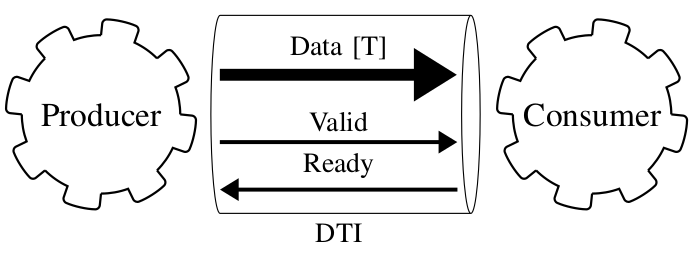
\includegraphics[width=0.5\linewidth]{dti}
  \caption{DTI interfejs\cite{PyGears_OSDA}}
  \label{DTI_intf_img}
\end{figure}

Jednostavan \textbf{\gls{dti}} interfejs se koristi za komunikaciju između gear-ova.
Modul koji šalje podatke se naziva Producer, a modul koji prima podatke se
naziva Consumer. \\
DTI se sastoji od sledećih signala:
\begin{itemize}
\item \textbf{Data} linije za podatke, proizvolje širine i proizvoljnog tipa.
\item \textbf{Valid} jednobitan signal kojim upravlja Producer i signalizira da
  je podataka na Data liniji validan.
\item \textbf{Ready} jednobitan signal kojim upravlja Consumer i signalizira da je
  konzumirao podatak sa Data linije i spreman za novi podatak.
\end{itemize}
Pomoću Valid i Ready signala realizovan je handshaking protokol. \\

\begin{figure}[H]
  \centering{
    \resizebox{0.75\textwidth}{!}{%
      \\
\begin{tikztimingtable}[%
    timing/dslope=0.1,
    timing/.style={x=5ex,y=2ex},
    x=5ex,
    timing/rowdist=4ex,
    timing/name/.style={font=\sffamily\scriptsize}
]
\busref{CLK}         & 18{c} \\
\busref{Data}      & 2u 3D 2U 1D 0L 1D 1U \\
\busref{Valid}   & 1L 3H 2L 2H L \\
\busref{Ready} & 3L 5H L  \\
\busref{Event}     & 3U 1D{ACK} 2U 1D{ACK} 1D{ACK} U\\
\extracode
\begin{pgfonlayer}{background}
\begin{scope}[semitransparent ,semithick]
\vertlines[darkgray,dotted]{0.5,1.5 ,...,8.0}
\foreach \i [count=\col from 0] in {0.5,1.5,...,8.0}
    \node[font=\scriptsize] at (\i,3) {${\col}$};
\end{scope}
\end{pgfonlayer}
\end{tikztimingtable}

    }}
  \caption{DTI primer transakcije}
  \label{dti_example1}
\end{figure}

Na slici(\ref{dti_example1}) prikazan je talasni oblik protokola:
\begin{enumerate}
\item Producer je postavio podatak na Data liniju i podigao Valid signal na
  jedinicu. Što označava validan podatak na magistrali.
\item Istog trenutka nakon postavljanja Valid signala na jedinicu Consumer može
  da koristi podatak na magistrali.
\item Consumer može koristiti podatak potreban broj taktova.
\item Kada Consumer završi sa korišćenjem podatka, postavlja Ready signal na
  jedinicu čime označava ACK(acknowledgment) odnosno signalizira da je završio
  sa podatkom na magistrali i da je spreman za sledeći podatak. \\
  Nakon handshake-a Producer može postaviti novi podatak na magistralu.
\item Producer ne sme menjati podatak na magistrali sve do pojave ACK od strane
  Consumera.
\item Producer može držati Valid signal na logičkoj nuli i tada se neće
  obavljati transakcije na magistrali.
\item Ne sme postojati kombinaciona putanja od Ready do Valid signala na strani
  Producer-a.
  Odnosno Producer ne sme odlučivati o postavljanju podatka na magistrali na
  osnovu stanja Consumer-a.
\item Može postojati kombinaciona putanja od Valid do Ready signala na strani
  Consumer-a.

\end{enumerate}

\subsection{Tipovi podataka} \label{pygears_data_types}

Data linija u DTI interfejsu pored toga što može biti proizvoljne širine može
predstavljati i različite kompleksne tipove podataka.
Ovim se omogućava bolja kompozicija modula, lakša manipulacija podacima,
pregledniji izvorni kod.

\subsubsection{Uint} \label{uint_sec}
\textbf{Uint[W]} predstavlja neoznačenu celobrojnu vrednost proizvoljne
širine W.

\subsubsection{Int} \label{int_sec}
\textbf{Int[W]} predstavlja označenu celobrojnu vrednost proizvoljne
  širine W.

\subsubsection{Tuple} \label{tuple_sec}
\textbf{Tuple[T1, T2, ..., TN]} predstavlja tip sličan strukturi gde
  polja Tn mogu biti bilo kog tipa. \\
  Koordinate piksela slike mogu se prigodno predstaviti kao Tuple tip. \\
  Na primer Tuple[Uint[W\_Y], Uint[W\_X]] ovaj Tuple sadrži dva Uint polja koji
  predstavljaju X i Y koordinate.

\subsubsection{Array} \label{array_sec}
\textbf{Array[T, N]} predstavlja niz od N podataka tipa T.

\subsubsection{Float}
\textbf{Float} se koristi za predstavljanje decimalnih brojeva pomoću formata
sa pokretnom tačkom.
Ovaj tip se koristi isključivo za simulaciju i ne može se implementirati u hardveru.

\subsubsection{Fixp}
\textbf{Fixp[WI, W]} se koristi za predstavljanje decimalnih brojeva sa fiksnom tačkom. \\
Format Fixed point tipa je \textbf{WI} širina celobrojnog dela i \textbf{W}
ukupna širina magistrale, širina decimalnog dela je razlika ove dve širine. \\
Ovaj tip se koristi za reprezentaciju decimalnih brojeva u hardveru.

\subsubsection{Queue} \label{queue_sec}
\textbf{Queue[T, LVL]} ili red predstavlja transakciju koja sadrži više
podataka proizvoljnog tipa T i informaciju o završetku transakcije EOT(end of
transaction).
Queue može biti proizvoljnog nivoa LVL. \\
Kao primer \textbf{Queue[Uint[4], 1](0, 1, 2, 3)} predstavlja red od četiri
četvorobitna podatka, primer talasnih oblika na slici ispod.
Rezultujuća Data magistrala biće širine 5 bita, 4 bita za podatak i 1 bit za EOT.

\begin{figure}[H]
  \centering{
    \resizebox{0.6\textwidth}{!}{%
      \\
\begin{tikztimingtable}[%
    timing/dslope=0.1,
    timing/.style={x=5ex,y=2ex},
    x=5ex,
    timing/rowdist=4ex,
    timing/name/.style={font=\sffamily\scriptsize}
]
\busref{CLK}         & 12{c} \\
\busref{Data}[4:0]      & 2u 1D{0x00} 1D{0x01} 1D{0x02} 1 D{0x13}  U \\
\busref{Data[3:0]} & 2u 1D{0} 1D{1} 1D{2} 1D{3} U \\
\busref{EOT\textsubscript{(Data[4])}} & U 3L 1H U \\
\busref{Valid}   & 1L 4H L \\
\busref{Ready} & 4L 1H L  \\
\busref{Event}     & 4U 1D{ACK} U \\
\extracode
\begin{pgfonlayer}{background}
\begin{scope}[semitransparent ,semithick]
\vertlines[darkgray,dotted]{0.5,1.5 ,...,6.0}
\foreach \i [count=\col from 0] in {0.5,1.5,...,6.0}
    \node[font=\scriptsize] at (\i,3) {${\col}$};
\end{scope}
\end{pgfonlayer}
\end{tikztimingtable}
    }}
  \caption{Primer transakcije tipa}
  \label{queue_img1}
\end{figure}

Dvodimenzionalna matrica se može predstaviti kao Queue[Uint[4], 2],
odnosno red nivoa 2 sa proizvoljnim podatkom u ovom slučajem četvorobitnim
neoznačnim brojem.

\begin{figure}[H]
  \centering{
    \resizebox{0.25\textwidth}{!}{%
      \begin{tikzpicture}
  % draw the grid and the numbers
  \draw (-1,-1) grid (2,2) foreach \i in {0,...,2}{
    (\i-.5,2.5) node{\i} (-1.5,1.5-\i) node{\i}};

  \node[text width=1.5cm] at (0.0,1.5) (A_coord) {\large \textbf{5}};
  \node[text width=1.5cm] at (1.0,1.5) (A_coord) {\large \textbf{1}};
  \node[text width=1.5cm] at (2.0,1.5) (A_coord) {\large \textbf{9}};

  \node[text width=1.5cm] at (0.0,0.5) (A_coord) {\large \textbf{3}};
  \node[text width=1.5cm] at (1.0,0.5) (A_coord) {\large \textbf{7}};
  \node[text width=1.5cm] at (2.0,0.5) (A_coord) {\large \textbf{11}};

  \node[text width=1.5cm] at (0.0,-0.5) (A_coord) {\large \textbf{0}};
  \node[text width=1.5cm] at (1.0,-0.5) (A_coord) {\large \textbf{4}};
  \node[text width=1.5cm] at (2.0,-0.5) (A_coord) {\large \textbf{15}};

\end{tikzpicture}

    }}
\caption{Matrica veličine 3x3}
\label{queue_matrix1}
\end{figure}

\begin{figure}[H]
\centering{
  \resizebox{.9\textwidth}{!}{%
    \\
\begin{tikztimingtable}[%
    timing/dslope=0.1,
    timing/.style={x=5ex,y=2ex},
    x=5ex,
    timing/rowdist=4ex,
    timing/name/.style={font=\sffamily\scriptsize}
]
\busref{CLK}         & 22{c} \\
\busref{Data}[5:0]      & 2u 1D{0x05} 1D{0x01} 1D{0x19} 1D{0x03} 1D{0x07}
1D{0x1B} 1D{0x00} 1D{0x04} 1D{0x1F} U \\
\busref{Data[3:0]} & 2u 1D{5} 1D{1} 1D{9} 1D{3} 1D{7} 1D{11} 1D{0} 1D{4} 1D{15}  U \\
\busref{EOT[1]\textsubscript{(Data[5])}} & U 6L 3H U \\
\busref{EOT[0]\textsubscript{(Data[4])}} & U 2L 1H 2L 1H 2L 1H U \\
\busref{Valid}   & 1L 9H L \\
\busref{Ready} & 9L 1H L  \\
\busref{Event}     & 9U 1D{ACK} U \\
\extracode
\begin{pgfonlayer}{background}
\begin{scope}[semitransparent ,semithick]
\vertlines[darkgray,dotted]{0.5,1.5 ,...,11.0}
\foreach \i [count=\col from 0] in {0.5,1.5,...,11.0}
    \node[font=\scriptsize] at (\i,3) {${\col}$};
\end{scope}
\end{pgfonlayer}
\end{tikztimingtable}

  }}
\caption{Transakcija matrice \ref{queue_matrix1}}
\label{queue_matrix2}
\end{figure}

Kao što se može videti linija za podatke je u ovom slučaju širine 6 bita, od
toga 2 bita su EOT. \\
Na slici(\ref{queue_matrix1}) u taktovima(3, 6, 9) niži bit EOT-a je na visokom nivou
što predstavlja podatak u poslednjoj koloni matrice.
U taktovima(7, 8, 9) viši bit EOT-a je na visokom nivou što označava podatke u poslednjoj
liniji matrice.
Konačno u taktu 9 oba EOT bita su na visokom nivou što označava poslednji podatak u matrici.

\subsubsection{Union} \label{union_sec}
\textbf{Union[T1, T2, ..., TN]} je unija koja može prenositi samo jedan od
  podataka Tn u trenutku.
  Uz podatak prenosi se i informacija o aktivnom podatku na magistrali.

\subsubsection{Unit} \label{unit_sec}
\textbf{Unit} je tip koji prenosi ``prazan'' podatak.

\begin{figure}[H]
\centering{
  \resizebox{.35\textwidth}{!}{%
    \\
\begin{tikztimingtable}[%
    timing/dslope=0.1,
    timing/.style={x=5ex,y=2ex},
    x=5ex,
    timing/rowdist=4ex,
    timing/name/.style={font=\sffamily\scriptsize}
]
\busref{CLK}         & 6{c} \\
\busref{Valid}   & 1L 1H L \\
\busref{Ready} & 1L 1H L  \\
\busref{Event}     & 1U 1D{ACK} U \\
\extracode
\begin{pgfonlayer}{background}
\begin{scope}[semitransparent ,semithick]
\vertlines[darkgray,dotted]{0.5,1.5 ,...,3.0}
\foreach \i [count=\col from 0] in {0.5,1.5,...,3.0}
    \node[font=\scriptsize] at (\i,3) {${\col}$};
\end{scope}
\end{pgfonlayer}
\end{tikztimingtable}
  }}
\caption{Unit tip}
\label{unit_img1}
\end{figure}

\subsection{Čistoća Gear-ova} \label{gear_purity}

Kako bi se gear-ovi lakše povezivali i njihova funkcionalnost i ponašanje bilo
razumljivo i predvidljivo dizajneru, preporučuje se pisanje ``čistih''  gear-ova. \\
``Čist'' gear je onaj čije je inicijalno stanje dobro poznato i koji će se nakon
izvršene funkcionalnosti potpuno vratiti u inicijalno stanje. \\
Čisto kombinacioni gear-ovi su uvek ``čisti''.

\newpage
\subsection{Definicija Gear komponenti}

PyGears trenutno podržava tri načina za implementaciju Gear komponenti.

\begin{code}[H]{python}{Primer definisanja Gear komponente}{gear_example1}
@gear
def gear_name(in1: T1, ..., inN: TN,
              *,
              p1=dflt, ..., pM=dfltM) -> ReturnType:
    # Gear implementation
\end{code}

Primer(\ref{gear_example1}) prikazuje definisanje gear komponente. \\
Dekorator \textbf{@gear} označava da je funkcija gear\_name zapravo Gear komponenta,
slično kao module ili entity kod Verilog-a i VHDL-a. \\
Kao parametri funkcije prosleđuju se DTI interfejsi i generički parametri.
Delimiter ``*'' označava početak generičkih parametara. \\

Ulazni DTI interfejsi mogu imati proizvoljan naziv i tipove opisane u
sekciji(\ref{pygears_data_types}). \\
Parametar može biti bilo koji Python objekat i može imati inicijalnu vrednost dflt.

\subsubsection{Gear implementiran pomoću SystemVerilog-a}

Jedan od mogućih načina implementacije Gear komponente je pisanje SystemVerilog
opisa pa zatim Python wrapper-a za komponentu. \\
Prilikom pisanja modula na ovaj način potrebno je pobrinuti se da napisana
komponenta poštuje DTI protokol kao i da je ``čist'' Gear(\ref{gear_purity}). \\

Prilikom pisanja wrapper-a za ovako implementiranu komponentu potrebno je
unapred odrediti ReturnType koji će odgovarati izlaznom interfejsu SystemVerilog modula. \\
Takođe deo za implementaciju Gear-a u Python-u može ostati prazan. \\

Kako postoji velika verovatnoća unošenja bagova u dizajn prilikom ručnog pisanja
modula koji poštuje DTI interfejs i koji je ``čist'', ovaj način implementacije
modula nije preporučen.

\subsubsection{Gear implementiram kompozicijom}

Kako PyGears dolazi sa bibliotekom osnovnih funkcionalnih modula, većina
potrebnih funkcionalnosti moguće je ostvariti njihovom kompozicijom. \\

\newpage

\subsubsection{Gear implementiram Python to HDL kompajlerom}

Moguće je i pisati opis gear-a u Python-u pomoću HDL kompajlera. \\

Kao primer prikazan je serialize gear koji kao ulaz prima niz podataka, a na
izlazu daje jedan po jedan podatak ulaznog niza, odnosno serializuje podatke.

\begin{code}[H]{python}{Primer kompajliranog serialize gear-a}{serialize_example}
@gear(svgen={'compile': True})
async def serialize(din: Array) -> b'din.dtype':
    async with din as val:
        for i in range(len(din.dtype)):
            yield val[i]
\end{code}

Kao primer možemo uzeti niz \textbf{Array[Uint[4], 3](3, 7, 9)} za očekivati je da će se
na izlazu pojaviti podaci redom 3, 7 pa 9 što je prikazano na slici \ref{serialize_example2}.
\begin{figure}[H]
\centering{
  \resizebox{.55\textwidth}{!}{%
    \\
\begin{tikztimingtable}[%
    timing/dslope=0.1,
    timing/.style={x=5ex,y=2ex},
    x=5ex,
    timing/rowdist=3ex,
    timing/name/.style={font=\sffamily\scriptsize}
]
\busref{CLK}         & 10{c} \\
\busref{din}      & 1U 3D{0x973} U \\
\busref{din[2]}      & 1U 3D{0x9} U \\
\busref{din[1]}      & 1U 3D{0x7} U \\
\busref{din[0]}      & 1U 3D{0x3} U \\
\busref{din\_valid}   & 1L 3H L \\
\busref{din\_ready} & 3L 1H L  \\
\busref{dout}      & 1U 1D{0x3} 1D{0x7} 1D{0x9} U \\
\busref{dout\_valid}   & 1L 3H L \\
\busref{dout\_ready} & 1L 3H L  \\
\extracode
\begin{pgfonlayer}{background}
\begin{scope}[semitransparent ,semithick]
\vertlines[darkgray,dotted]{0.5,1.5 ,...,4.0}
\foreach \i [count=\col from 0] in {0.5,1.5,...,4.0}
    \node[font=\scriptsize] at (\i,3) {${\col}$};
\end{scope}
\end{pgfonlayer}
\end{tikztimingtable}

  }}
\caption{Serialize gear primer}
\label{serialize_example2}
\end{figure}

\newpage

\section{Integracija IP jezgra sa Zynq sistemom}

PyGears i SystemVerilog implementacije predložene arhitekture su kompatibilne u
pogledu spoljnih interfejsa.
Pored toga ove implementacije su uveliko nezavisne od ciljane tehnologije za
implementaciju. \\
U ovom radu IP jezgro će biti implementirano na Zynq \gls{soc} sistemu. \\

Korišćeni DTI interfejs je kompatibilan sa AXI-Stream intefejsom, tako da je
integracija sa sistemima koji koriste druge interfejse poput Avalon-a trebala
biti jednostavna uz adaptere. \\

Preporučena je integracija IP jezgra u sistem sa procesorom, što će biti i
prikazano u ovom radu.
U ovom slučaju biće korišćen ARM Cortex-A9 procesor koji se može naći kao Hard
IP jezgro unutar Zynq SoC platforme kompanije Xilinx. \\

\subsection{Zynq}

Zynq se sastoji od \gls{ps} sistem i \gls{pl} sistema.
PS sistem je sačinjen od već pomenutog ARM Cortex-A9 \gls{APU} procesora.
Dok PL sistem predstavlja \gls{fpga} programabilnu logiku Artix-7 familije. \\

Komunikacija između PL i PS sistema se obavlja preko \gls{axi} interfejsa,
interapt pinova ili \gls{emio} pinova.\\

ARM procesor ima mogućnost povezivanja eksterne \gls{ddr} memorije preko
internog DDR kontrolera.
Preko ovog kontrolera pristup memoriji ima i PL sistem. \\
Zynq SoC ima podršku GNU/Linux operativnog sistema.

\newpage

\subsection{Predloženi blok dijagram sistema}

U nastavku je prikazan okviran blok dijagram povezivanja projektovanog IP jezgra
sa procesorskim sistemom. \\
Na slici su izostavljene interkonekcijske komponente, generatori reset i clk signala,
memorijske konekcije itd... \\

\begin{figure}[H]
  \centering
  \resizebox{1\textwidth}{!}{%
    \pgfdeclarelayer{background1}
\pgfdeclarelayer{background2}
\pgfdeclarelayer{foreground}
\pgfsetlayers{background1, background2,main,foreground}

\tikzstyle{cloud1} = [draw=black, thick, fill=red!20, minimum height = 1em]
\tikzstyle{block_l} =[draw, text centered, fill=blue!15, minimum width=2.5cm, minimum height=2.5cm]
\tikzstyle{block_m} =[draw, text centered, fill=blue!15, minimum width=2.0cm, minimum height=1.0cm]
\tikzstyle{block_s} =[draw, text centered, fill=blue!15, minimum width=2cm, minimum height=1.5cm]
\tikzstyle{line} = [draw, line width = 0.05cm, arrows={-Triangle[length=0.2cm]}]

\tikzstyle{dreg} = [draw, text centered, fill=blue!15, minimum width = 1.5cm,
minimum height=1.5cm]

\tikzstyle{square} = [draw, thick, fill=blue!15, circle, minimum size = 1cm, node distance = 2cm]
\tikzstyle{mult} = [draw, thick, fill=blue!15, circle, minimum size = 1cm ,node distance = 2cm]
\tikzstyle{sum} = [draw, thick, fill=blue!15, circle, minimum size= 1cm, node distance = 2cm]

\begin{tikzpicture}[thick]

  \node [block_l, fill=red!20] (csc_cls) {\textbf{\large cascade\_classifier}};
  \node [coordinate, left = 0cm of csc_cls] (csc_cls_in){};
  \node [coordinate, left = 2cm of csc_cls_in] (ii_in){};
  \node [coordinate, above right = -0.5cm and 0cm of csc_cls] (csc_cls_out){};
  \node [coordinate, below right = -0.5cm and 0cm of csc_cls] (csc_cls_irq){};
  \node [coordinate, right = 1cm of csc_cls_irq] (csc_cls_irq1){};

  \node [block_l, fill=red!20, below = 2cm of csc_cls] (dm_cmd) {\textbf{\large dm\_cmd}};
  \node [coordinate, below left = 0 and -0.5cm of dm_cmd] (dm_cmd_in){};
  \node [coordinate, below right = 0 and -0.5cm of dm_cmd] (dm_cmd_irq_out){};
  \node [coordinate, above right = 0cm and -0.5cm of dm_cmd] (dm_cmd_irq_in){};
  \node [coordinate, above = 1cm of dm_cmd_irq_in] (dm_cmd_irq_in1){};
  \node [coordinate, left = 0cm of dm_cmd] (mm2s_cmd){};
  \node [coordinate, right = 0cm of dm_cmd] (s2mm_cmd){};

  \node [block_l, below = 2cm of dm_cmd] (apu) {\textbf{\large APU}};
  \node [coordinate, above left = 0cm and -0.5cm of apu] (apu_cmd){};
  \node [coordinate, above right = 0cm and -0.5cm of apu] (apu_irq){};
  \node [coordinate, left = 0cm of apu] (apu_mm2s){};
  \node [coordinate, right = 0cm of apu] (apu_s2mm){};

  \node [block_l, right = 3cm of csc_cls] (s2mm) {\textbf{\large dm\_s2mm}};
  \node [coordinate, right = 0cm of s2mm] (s2mm_out){};
  \node [coordinate, right = 1cm of s2mm] (s2mm_out1){};
  \node [coordinate, above left = -0.5cm and 0cm of s2mm] (s2mm_in){};
  \node [coordinate, below left = -0.5cm and 0cm of s2mm] (s2mm_cfg){};
  \node [coordinate, left = 1cm of s2mm_cfg] (s2mm_cfg1){};


  \node [block_l, left = 2cm of csc_cls] (mm2s) {\textbf{\large dm\_mm2s}};
  \node [coordinate, above left = -0.5cm and 0cm of mm2s] (mm2s_in){};
  \node [coordinate, left = 2cm of mm2s_in] (mm2s_in1){};
  \node [coordinate, below left = -0.5cm and 0cm of mm2s] (mm2s_cfg){};
  \node [coordinate, left = 1cm of mm2s_cfg] (mm2s_cfg1){};
  \node [coordinate, right = 0cm of mm2s] (mm2s_out){};

  %% group %%
 \begin{pgfonlayer}{background1}
   \node[inner sep=20pt, fill=yellow!25, rounded corners, draw, thick,fit=(csc_cls) (s2mm_out1) (mm2s_in1) (dm_cmd) (mm2s) (s2mm) (apu)] (system) {};
  \node[above left] at (system.south east) {\huge \textbf{SoC}};
\end{pgfonlayer}


  % arrows
  \path [line] (csc_cls_out) node[transition, yshift=+0.3cm, xshift=+1.3cm] {detect\_addr}  -- (s2mm_in);
  \path [line] (mm2s_out) -- (csc_cls_in) node[transition, yshift=+0.3cm, xshift=-0.8cm] {img\_in}  ;
  \path[line] (csc_cls_irq) node[transition, yshift=+0.3cm, xshift=+0.6cm] {irq}  -- (csc_cls_irq1) |- (dm_cmd_irq_in1) -- (dm_cmd_irq_in);

  \path [line] (s2mm_cmd) node[transition, yshift=+0.3cm, xshift=+1.0cm] {s2mm\_cfg} -| (s2mm_cfg1) -- (s2mm_cfg);
  \path [line] (mm2s_cmd) node[transition, yshift=+0.3cm, xshift=-1.0cm] {mm2s\_cfg} -| (mm2s_cfg1) -- (mm2s_cfg);

  \path[line] (s2mm_out) node[transition, yshift=+0.3cm, xshift=+0.8cm] {s2mm}  -- (s2mm_out1) |- (apu_s2mm);

  \path[line] (apu_mm2s) node[transition, yshift=+0.3cm, xshift=-0.8cm] {mm2s} -| (mm2s_in1) -- (mm2s_in);

  \path[line] (apu_cmd) node[transition, yshift=+0.5cm, xshift=-1.0cm] {apu\_cmd}  -- (dm_cmd_in);

  \path[line] (dm_cmd_irq_out) node[transition, yshift=-0.5cm, xshift=+0.4cm] {irq}  -- (apu_irq);


\end{tikzpicture}
  }
  \caption{Okviran blok dijagram sistema.}
  \label{system_bd_approx}
\end{figure}

Blokovi obojeni crvenom bojom su projektovani u okviru ovog rada.
Blokovi obojeni plavom bojom su standardne komponente i mogu se naći u okviru
softverskog alata od proizvođača korišćenog SoC-a. \\

Kako je već rečeno spoljni interfejsi \textbf{cascade\_classifier} IP jezgro su
Streaming tipa.
Streaming interfejsi nemaju informaciju o adresi, tako da sa njima nije
moguće adresirati podatak iz DDR memorije preko DDR kontrolera. \\

Komponente dm\_s2mm i dm\_mm2s su Data Mover-i, koji pretvaraju Streaming interfejs u \gls{mm}
interfejse.
Kako Streaming interfejs prenosi samo podatak i nema informaciju o
adresi, potrebno je proslediti adresu i broj podataka preko posebnog komandnog
interfejsa, na ovoj slici to su s2mm\_cfg i mm2s\_cfg.\\

Glavno IP jezgro nema koristi od informacije sa koje adrese dolazi slika i na
kojoj adresi se smeštaju rezultati, pa je zato za generisanje komande za Data Mover
komponente zadužen dm\_cmd.\\
Komponenta dm\_cmd od procesora dobija adresu bafera slike i rezultata iz eksterne DDR
memorije i na osnovu toga generiše komande za Data Mover-e. \\
Procesor adrese i broj podataka šalje preko apu\_cmd interfejsa. \\

Nakon konfigurisanja Data Mover-a prvo će sa radom početi dm\_mm2s Data Mover,
koji će poslati zahtev za sliku DDR kontroleru i pročitane podatke proslediti
glavnom IP jezgru na obradu.
Nakon popunjavanja IMG RAM memoriju unutar glavnog IP jezgra, jezgro počinje
obradu slike. \\

Ukoliko dođe do detekcije objekta na nekoj koordinati, ta koordinata će biti
poslata preko dm\_s2mm Data Mover-a u određenu lokaciju za smeštanje rezultata u
okviru eksterne DDR memorije. \\

Nakon završetka obrade trenutne slike aktiviraće se irq signal koji označava
interrupt za procesor.
Glavno IP jezgro će držati aktivnim ovaj signal samo jedan takt, dok će se taj
signal sačuvati u registru u okviru dm\_cmd jezgra i biće prosleđen na izlazni
irq signal povezan sa procesorom. \\
Nakon što procesor detektuje interrupt signal, to je znak procesoru da može da
pripremi sledeću sliku.
Nakon smeštanja naredne slike u bafer procesor treba da resetuje registrovani
interrupt u okviru dm\_cmd jezgra, to radi slanjem komande preko apu\_cmd
interfejsa. \\
Nakon resetovanja interrupt signala, procesor ponovo šalje zahtev za obradu
slike. \\

Procesor pored slanja komande IP jezgru treba da preuzme sliku sa kamere ili
učita iz fajla, zatim je konvertuje u grayscale reprezentaciju.
Rezultate detekcije procesor može koristiti za željeni zadatak. \\

\newpage

\subsection{Implementirani sistem na Zynq SoC}

U ovom radu sistem je implementiran na Zynq-7020 SoC.
Korišćena je ZTurn\cite{zturn} ploča firme MYiR.
Ova ploča se sastoji od Zynq-7020 čipa, 1GB eksterne DDR3 memorije, \gls{hdmi}
kontroler i konektor, tasteri i \gls{led} za testiranje, g-senzor, temperaturni
senzor, buzzer, flash memorija, SD card socket, Gig ethernet, JTAG, USB, CAN itd...
Što se može videti na sledećoj slici. \\

\begin{figure}[H]
  \centering
  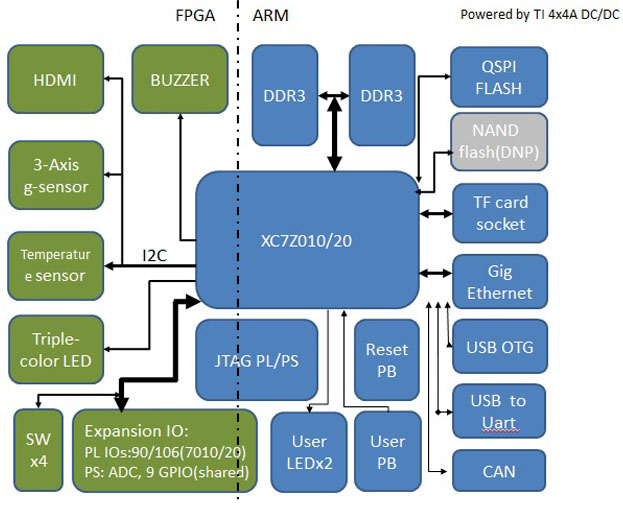
\includegraphics[width=0.65\linewidth]{images/zturn.jpg}
  \caption{Zturn ploča\cite{zturn}}
  \label{zturn_bd}
\end{figure}



Od eksternih periferija u ovom projektu korišćeni su SD kartica, Ethernet, HDMI,
USB i DDR memorija.
Procesor izvršava Arch Linux\cite{arch} operativni sistem, a komunikacija sa IP jezgrom je
odrađena preko napisanog Linux Kernel Drivera i korisničke aplikacije. \\

Na sledećoj strani prikazan je blok dijagram integratora implementiranog
sistema. \\
Može se primetiti da pored komentarisanih komponenti za povezivanje procesora sa
IP jezgrom, na blok dijagramu se nalazi i Video kontroler pod nazivom
hdmi\_core.
Ovo jezgro se koristi za slanje sadržaja framebuffer-a Linux Kernel-a na
eksterni HDMI kontroler, u cilju grafičkog interfejsa korisničke aplikacije. \\

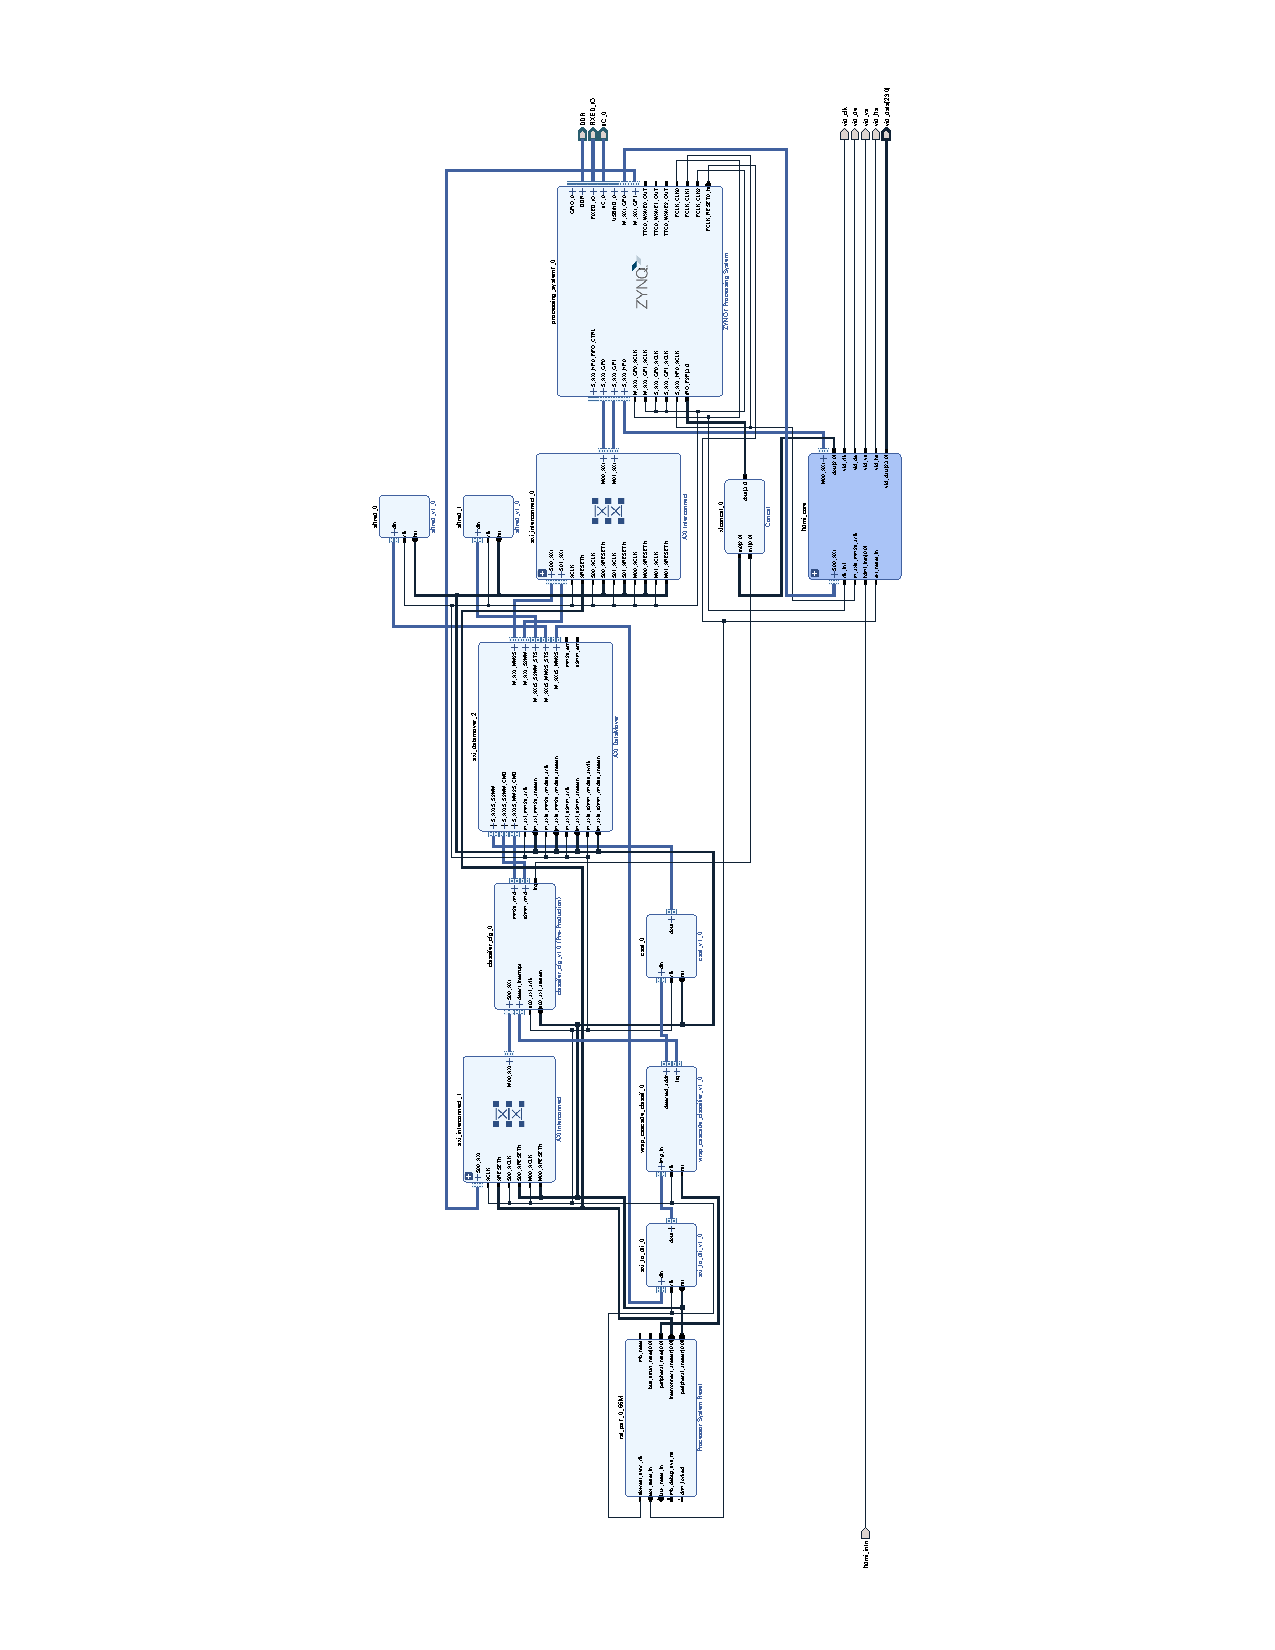
\includepdf[pages=-,pagecommand={},width=1.6\textwidth, height=1.2\textheight]{images/system_bd.pdf}


\subsection{Rezultati implementacije sistema}

\subsubsection{Sinteza i implementacija hardvera}
FPGA čipovi se sastoje od velikog broja programabilnih primitivnih blokova i
mreže za rutiranje.
Ove blokove je potrebno konfigurisati i međusobno ih povezati kako bi se dobila
željena funkcionalnost.
Kako se tipični dizajnovi koji ciljaju FPGA čipove sastoje od desetina hiljada
LUT-ova i ostalih komponenti, ovaj korak nije moguće odraditi ručno.
Sintezu i implementaciju digitalnog hardvera je jedino moguće uraditi pomoću
automatskog alata. \\

Proizvođači FPGA čipova uglavnom imaju svoj softverski alat za obavljanje ove
radnje.
Tako u slučaju Xilinx FPGA čipova potrebno je koristiti Vivado.\\

Prilikom sinteze hardvera alat hijerarhijski struktruirane HDL modele izravna i
napravi model sa istom hijerarhijom sačuvan u formatu netliste.
Tokom sinteze se rade i razne optimizacije poput deljenja funkcionalnih resursa,
logička minimizacija, optimizacija mašina stanja itd...
Konačno alat za sintezu može mapirati komponente generisane netliste u
primitivne blokove ciljane FPGA arhitekture, tzv Technology Mapping. \\
Nakon koraka sinteze moguće je proceniti koliko će se hardverskih primitivnih
blokova koristiti u konačnoj hardverskoj implementaciji. \\
Na osnovu toga se može zaključiti da li implementirani hardver zadovoljava
ograničenja potrošnje resursa. \\

Nakon sinteze hardvera potrebno je odraditi Place and Route komponenti na
željenom FPGA čipu.
To je takođe moguće odraditi automatskim alatom.
Nakon ovog koraka moguća je procena vremenskih karakteristika implementiranog
hardvera.
Pošto su poznata kašnjenja primitivnih blokova i moguća je estimacija kašnjenja
mreže za rutiranje može se proceniti da li će dizajn zadovoljavati vremenska
ograničenja. \\
Takođe moguće je proceniti i potrošnju konačne implementacije. \\

Pored zvaničnih alata za sintezu i implementaciju digitalnog hardvera na FPGA
čipovima, postoje i alternativna Open Source rešenja.
Problem sinteze rešava alat pod nazivom yosys\cite{yosys}, ovaj alat je brži od
zvaničnih alata za sintezu, uz to u nekim slučajevima generiše optimalniji
hardver, dok je manje efikasan u mapiranju hardvera na tehnologiju. \\
Za Place and Route može se koristiti nextpnr\cite{nextpnr}.
Pored toga postoji projekat SymbiFlow\cite{symbiflow} koji nastoji da poveže sve
ove alate i obezbedi jedinstveni alat za implementaciju digitalnog hardvera na
FPGA čipove nezavisno od proizvođača.
Veliki problem u ovom projektu predstavlja što FPGA proizvođači ne objavljuju
javno arhitekturu čipova i format Bitstream-a, pa se do ovih informacija mora
doći reverznim inženjeringom. \\

\newpage

\subsubsection{Analiza potrošnje hardverskih resursa}

U narednoj tabeli biće prikazano zauzeće hardverskih resursa u slučaju PyGears
implementacije.
Biće prikazana potrošnja samo glavnog IP jezgra i ukupnog sistema. \\

\newcolumntype{P}[1]{>{\centering\arraybackslash}p{#1}}
\begin{center}
  \centering
  \captionof{table}{Hardverski resursi nakon sinteze}
  \begin{tabular}{| P{3cm} | P{3cm} | P{3cm} | P{3cm} | P{3cm} | P{3cm} |}
    \hline
    Name  & LUT & FF & BRAM & DSP  \\ \hline
    Total & 14,259 (27\%) & 14,033 (13\%) & 47.5 (34\%) & 7 (3\%)  \\ \hline
    Cascade Classifier & 6,216 (12\%) & 2,252 (2\%) & 35 (25\%) & 7 (3\%) \\ \hline
  \end{tabular}
\end{center}

Nakon implementacije dobijaju se oko 10\% niže brojke za LUT i FF komponente. \\
Kao što se može videti najkritičniji deo ovog IP jezgra je broj korišćenih BRAM
komponenti što je bilo i očekivano na osnovu analize predložene arhitekture. \\
Može se videti da je projektovano jezgro veoma efikasno u pogledu ostalih
hardverskih resursa i ostaje prostora za ubrzanje dodavanjem hardverskih
resursa, odnosno paralelizma.

\subsubsection{Analiza vremenskog izveštaja i Timing Closure}

Frekvencija takta je bitna stavka, što većom frekvencijom taktujemo IP jezgro
brzina obrade slike će biti brža.
Naravno postoji ograničenje maksimalne frekvencije koja se može postići.
Ovo ograničenje postoji zbog kašnjenja logičkih blokova i mreže za rutiranje unutar FPGA čipa.
Izlazni signali flip flopova prolaze kroz kombinacionu logiku i dolaze do ulaza
sledećeg flip flopa, kašnjenje ove putanje mora biti kraće od periode takta uz
dodatan uticaj Setup i Hold vremena flip flopova.

\begin{figure}[H]
  \centering
  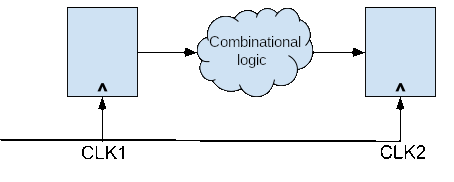
\includegraphics[width=0.55\linewidth]{images/comb.png}
  \caption{Kašnjenje kombinacione logike}
  \label{comb_logic}
\end{figure}

Mreža kombinacione logike predstavljena oblačićem može imati značajno vreme
propagacije.
Jedan od načina da se vreme propagacije smanji je ubacivanjem registara unutar
kombinacione mreže. \\
To je ujedno i najčešća tehnika ubrzavanja dizajna u krajnjoj fazi i
zadovoljavanja vremenskih ograničenja dizajna, takozvani Timing Closure. \\

\newpage

Nakon podešavanja takta na 47MHz i pokretanja implementacije može se videti da
su vremena zadovoljena za odabrani takt. \\
Empirijski se može zaključiti da frekvencija sistema srednje veličine
implementiranog na Zynq-7020 čipu može dostići brzine do oko 110MHz, na osnovu
čega možemo zaključiti da se u ovom slučaju mogu postići bolji
rezultati. \\
Na slici ispod su prikazane najkritičnije putanje u okviru dizajna. \\

\begin{figure}[H]
  \centering
  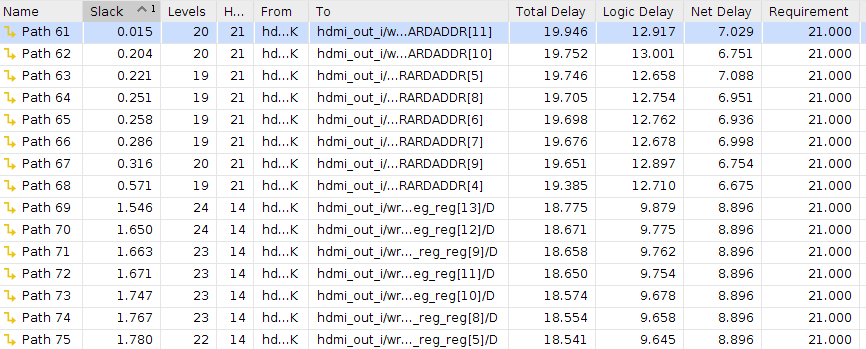
\includegraphics[width=1\linewidth]{results/implementation/pygears_slow/timing.png}
  \caption{Vremenski izveštaj pre skraćivanja kombinacionih putanja}
  \label{slow_time}
\end{figure}

Takođe može se i primetiti da je Logic Delay koji predstavlja vreme propagacije
kroz kombinacionu logiku veće od Net Delay-a koji predstavlja vreme
propagacije kroz mrežu za rutiranje.
Na Net Delay se ne može mnogo uticati i uveliko zavisi od kvaliteta korišćenog
FPGA čipa. \\

Može se primetiti veliko odstupanje između prvih desetak najkritičnijih putanja,
kao i da su putanje koje imaju Logic Delay od približno 13ns grupisane u okviru
jednog interfejsa.
To je znak da postoje putanje koje imaju značajno duže vreme propagacije od
ostatka sistema, pa je njih potrebno ubrzati. \\
Pomoću Vivado alata moguće je identifikovati putanju propagacije kritičnih
putanja i odlučiti gde bi se kombinaciona putanja mogla prekinuti i ubaciti
registar.
Ovo je dugotrajan proces i mora se raditi iz više iteracija, nakon svakog
ubacivanja registara mora se verifikovati funkcionalna ispravnost sistema, zatim
se ponovo pokreće implementacija. \\
U svakoj narednoj iteraciji sve je teže uočiti kritične putanje. \\

\newpage

PyGears dodatno olakšava proces skraćivanja kombinacionih putanja jednostavnim
ubacivanjem registara u dizajn što je prikazano na sledećem primeru. \\

\lstinputlisting[language=Python, mathescape, caption={PyGears implementacija
  stddev komponente}, captionpos=t, label=stddev_pygears]{examples/speedup.py}

U kodnom segmentu iznad u liniji 5 importuje se gear dreg koji predstavlja
registar i lokalno se naziva dreg\_sp.
Ovo može biti koristan detalj jer pomaže u boljoj distinkciji između registara
koji su prisutni funkcionalno i onih koji su ubačeni radi skraćivanja
kombinacionih putanja. \\
U linijama 12 i 15 može se videti skraćivanja kombinacione putanje posle
frame\_sum gear-a ubacivanje dreg\_sp gear-a. \\

Dodatna prednost PyGears-a u ovoj situaciji je činjenica da se ubacivanjem
registara unutar dizajna ne može izgubiti funkcionalna korektnost sistema.
Iako se ne može izgubiti funkcionalna korektnost, nasumičnim ubacivanjem
registara se može pogoršati vremenske performanse.
Prilikom ubacivanja registara može doći do gubljenja balansa između dve
paralelne grane, pa će jedan podatak uvek kasniti jedan takt do sinhronizacionog
gear-a u odnosu na drugu granu, usled čega će se na izlazu sinhronizacionog
gear-a pojaviti neželjeni takt pauze.
Pažljivom analizom paralelnih grana i sinhronizacionih tačaka, moguće je
balansirati grane dodavanjem dodatnog registra u nebalansiranoj grani. \\

\newpage

Konačno nakon skraćivanja kombinacionih putanja dostignuta je frekvencija takta
od 100MHz.\\
Pored skraćivanja kombinacionih putanja dodatno je uključena i
Performance ExplorePostRoutePhysOpt strategija za implementaciju u okviru
Vivado alat, ova strategija će učiniti da vreme implementacije traje duže, ali
će se kao rezultat dobiti implementacija sa boljim vremenskim karakteristikama,
ponekad sa cenom dodatnih hardverskih resursa. \\

Kao što se može videti dostignuto je više nego duplo ubrzanje sistema ovom tehnikom. \\
Treba napomenuti da je u RTL metodologiji preporučljivo voditi računa o
kombinacionim putanjama u ranijim fazama implementacije, dok je zbog lakog
ubacivanja registara u kasnijim fazama dizajna u PyGears metodologiji
pogodniji ovakav pristup. \\

\begin{figure}[H]
  \centering
  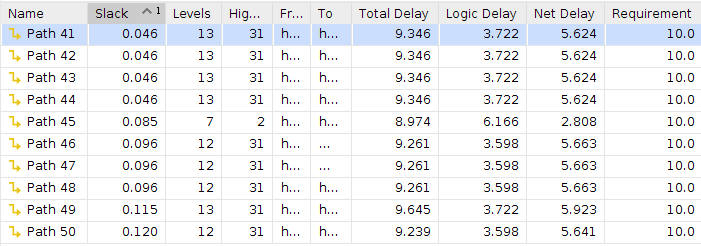
\includegraphics[width=1\linewidth]{results/implementation/pygears_fast/timing.png}
  \caption{Vremenski izveštaj posle skraćivanja kombinacionih putanja}
  \label{slow_time}
\end{figure}

Može se primetiti da je dostignuto ogromno skraćenje Logic Delay vremena, a
može se  primetiti i da je Net Delay značajno skraćen to je verovatno rezultat
lakšeg zadatka za Place and Route alat nakon ubacivanja registara. \\
Na slici je prikazano 10 kombinacionih putanja u prošlom slučaju smo primetili
veliku razliku ukupnog kašnjenja u istom broju putanja, u ovom slučaju ne bismo
primetili veliku razliku u totalnom kašnjenju čak i kod prvih 100 kritičnih
putanja, to je pokazatelj da se dolazi do granica mogućnosti ubrzavanja sistema
ovim pristupom. \\
U tom trenutku dolazimo do Timing Closure-a, kada smo zadovoljni sa vremenskim
karakteristikama sistema. \\

\subsection{Softver procesora}

Nakon što je isprojektovan i implementiran sistem, potrebno je napisati
softver za procesor koji će konfigurisati IP jezgro i koristiti rezultate detekcije.
Ovde postoji izbor da li će procesor izvršavati operativni sistem ili će izvršavati
Bare Metal aplikaciju. \\

Prednosti Bare Metal aplikacije je veća pouzdanost, jednostavnost i bolje performanse zbog
nepostojanja schedule-inga. \\
Prednosti operativnog sistema je brži i lakši razvoj aplikacije, nezavisnost
aplikacije od platforme, laka implementacija korisničkog interfejsa,
lak pristup internetu itd...\\

U ovom radu je odlučeno da procesor radi na GNU/Linux operativnom sistemu. \\
Softver je particionisa na sledeći način:

\begin{figure}[H]
  \centering
  \resizebox{0.9\textwidth}{!}{%
    \pgfdeclarelayer{background1}
\pgfdeclarelayer{background2}
\pgfdeclarelayer{foreground}
\pgfsetlayers{background1, background2,main,foreground}

\tikzstyle{cloud1} = [draw=black, thick, fill=purple!20, minimum height = 1em]
\tikzstyle{block_l} =[draw, text centered, fill=blue!15, minimum width=2.5cm, minimum height=1.5cm]
\tikzstyle{block_m} =[draw, text centered, fill=blue!15, minimum width=2.0cm, text width=2.0cm, minimum height=1.0cm]
\tikzstyle{block_s} =[draw, text centered, fill=blue!15, minimum width=2cm, minimum height=1.5cm]
\tikzstyle{line} = [draw, arrows={-Triangle[length=0.2cm]}]

\tikzset{
  multiplexer/.style={
    draw,
    trapezium,
    fill=blue!15,
    shape border uses incircle,
    shape border rotate=180,
    minimum size=25pt
  }
}

\begin{tikzpicture}[thick]

  \node [block_m] (c_user) {User C};
  \node[coordinate, above = 0cm of c_user] (c_in);
  \node[coordinate, above = 0.5cm of c_in] (c_in1);
  \node[coordinate, below left = 0cm and -0.5cm of c_user] (c_write);
  \node[coordinate, below = 0cm of c_user] (c_read);
  \node[coordinate, below right = 0cm and -0.5cm of c_user] (c_mmap);

  \node [block_m, above left = 1cm and 0.25cm of c_user] (python) {Python};
  \node[coordinate, below = 0cm of python] (python_out);
  \node[coordinate, below = 0.5cm of python] (python_out1);

  \node [block_m, above right = 1cm and 0.25 of c_user] (cpp) {C++};
  \node[coordinate, below = 0cm of cpp] (cpp_out);
  \node[coordinate, below = 0.5cm of cpp] (cpp_out1);

  \node [block_l, fill=red!20, below = 1.5cm of c_user] (drv) {Device Driver};
  \node[coordinate, above left = 0cm and -0.5cm of drv] (drv_write);
  \node[coordinate, above = 0cm of drv] (drv_read);
  \node[coordinate, above right = 0cm and -0.5cm of drv] (drv_mmap);
  \node[coordinate, below = 0cm of drv] (drv_out);

  \node[coordinate, below left = 0.5cm and 4cm of c_user] (dot_start);
  \node[coordinate, below right = 0.5cm and 4cm of c_user] (dot_end);

  \draw [dashed] (dot_start) node[transition, yshift=-.3cm, xshift=+1.6cm]{Kernel Space} node[transition, yshift=0.3cm, xshift=+1.6cm]{User Space} -- (dot_end);


  \node[coordinate, below left = 0.5cm and 4cm of drv] (hw_dot_start);
  \node[coordinate, below right = 0.5cm and 4cm of drv] (hw_dot_end);

  \draw [dashed] (hw_dot_start) node[transition, yshift=-.3cm, xshift=+1.6cm]{FPGA} -- (hw_dot_end);

  % paths
  \path [line, very thick] (python_out) -- (python_out1) -| (c_in1) -- (c_in);
  \path [line, very thick] (cpp_out) -- (cpp_out1) -| (c_in1) -- (c_in);

  \path [line, very thick] (c_write) -- (drv_write);
  \path [line, very thick] (drv_read) -- (c_read);
  \path [line, very thick] (c_mmap) -- (drv_mmap);

  \path [line, very thick] (drv_out) -- +(0, -1.5cm);
  \path [line, very thick] (drv_out) -- +(0, -1.5cm) -- (drv_out);
  % \path [line, very thick] (w_sum_in) node[transition, yshift=+0.3cm, xshift=0.6cm] {\textbf{weight\_data}}  node[transition, yshift=-0.3cm, xshift=-0.0cm] {\textbf{fb\_ii}}  -- (w_sum1_in_port);

\end{tikzpicture}
  }
  \caption{Softverski stek.}
  \label{software_stack}
\end{figure}

Kernel Device driver šalje komande dm\_cmd komponenti preko AXI Lite interfejsa.
Komunikacija između drajvera i AXI Lite komponente se obavlja preko memorijskog
mapiranja.
Registri unutar dm\_cmd komponente su mapirani na određenu memorijsku lokaciju u
okviru adresnog prostora procesora.
Procesor može pristupati ovim registrima prostim upisivanjem na adresi mapiranih registara.\\
Pored toga interrupt signal koji označava kraj obrade slike se obrađuje unutar
Kernel drajvera. \\
Kernel drajver ima implementirane sledeće operacije:
\begin {itemize}
  \item \textbf{Write} operacija startuje IP jezgro upisivanjem potrebnih adresa
    u dm\_cmd komponentu i postavlja bit za start na jedinicu. \\
  \item \textbf{Read} operacija vraća sadržaj bafera za rezultate korisničkoj
    aplikaciji. \\
  \item \textbf{Mmap} operacija memorijski mapira bafer slike iz korisničke
    aplikacije na fizički kontinualni memorijski bafer unutar kernel prostora.
    Fizičku adresu kontinualnog memorijskog bafera je potrebno poslati dm\_cmd
    komponenti unutar Write operacije.\\
\end{itemize}

Prilikom završetka obrade slike poslaće se zahtev za interapt procesoru,
taj zahtev će se obraditi u okviru Kernel drajvera.
Nakon pojave interapta poslaće se komanda za resetovanje interapt registra u
okviru dm\_cmd komponente, zatim će se otključati
read\_mutex kako bi se omogućila operacija Read. \\

Korisnička aplikacija je podeljena u dva nivoa.
Niži nivo aplikacije predstavlja C funkciju koja je zadužena za komunikaciju sa
kernel drajverom.
Ova funkcija obavlja operacije čitanja rezultata i memorijskog mapiranja prosleđene slike na
kernel memorijski bafer.
Funkciju je moguće kompajlirati kao \gls{so} biblioteku tako da je moguć pristup
iz Python-a preko ctypes biblioteke, kao i pristup iz C++-a. \\

Viši nivoi korisničke aplikacije mogu biti napisani u programskim jezicima višeg
nivoa.
U ovom radu je napisana aplikaciju u Python jeziku.
Prednost korišćenja jezika kao što je Python je jednostavno korišćenje
biblioteka poput OpenCV-a.
Pomoću OpenCV biblioteke može se na lak način pročitati slika iz fajla ili
preuzeti frejm sa kamere, zatim pretvoriti u grayscale reprezentaciju. \\
Takođe kao vizualizaciju rada IP jezgra u okviru OpenCV biblioteke može se na
lak način nacrtati pravougaonici na pozicijama detektovanih objekata. \\


\newpage
\section{Performanse i optimizacije}

\subsection{Performanse}

Performanse projektovanog IP jezgra biće upoređene sa softverskim
implementacijama.
Porediće se C++ specifikacija napisana u ovom radu, OpenCV implementacija i
hardverska implementacija. \\
Mereno je samo vreme izvršavanja detekcije, odnosno isti zadatak koji obavlja IP
jezgro obalja i softver.
OpenCV implementacija biće poređena sa automatskim skaliranjem slike i sa
fiksnim faktorom skaliranja korišćenim u hardverskoj implementaciji. \\
Poređene platforme su Ryzen 5 1600 procesor pod Arch Linux-om, Thinkpad T430s
i5-3210m pod Arch Linux-om i Zynq 7020 pod Arch Linux ARM-om. \\

U sledećoj tabeli je prikazano prosečno vreme detekcije na Caltech dataset-u
slika veličine 240x320.

\renewcommand{\arraystretch}{1.5}
\newcolumntype{P}[1]{>{\centering\arraybackslash}p{#1}}
\begin{center}
  \centering
  \captionof{table}{Poređenje performansi}
  \begin{tabular}{| P{2cm} | P{2.5cm} | P{2.5cm} | P{2.5cm} | P{2.5cm} |}
    \hline
    Platform & OpenCV Scaling Auto & OpenCV Scaling Fixed & C++ Spec & IP Core \\ \hline
    \hline
    Zynq & 571 ms & 205 ms & 3593 ms & 926 ms \\ \hline
    Thinkpad & 28 ms & 10.3 ms & 194 ms & N/A \\ \hline
    Ryzen & 22.8 ms & 9.7 ms & 192 ms & N/A \\ \hline
  \end{tabular}
\end{center}

Kao što je bilo i očekivano OpenCV implementacija pod Ryzen procesorom ima
najkraće vreme izvršavanja.
Može se videti da iako Ryzen procesor ima 6 bržih CPU jezgara za razliku od 2 kod
Thinkpad laptopa ne postoje drastične razlike u vremenu izvršavanja softverskih
implementacija. \\
Zynq je očekivano najsporiji od tri platforme.
Projektovano IP jezgro je 4.5 puta sporije od OpenCV implementacije na istoj
platformi. \\

Iako su performanse IP jezgra slabije od OpenCV implementacije treba uzeti u
obzir i odnos frekvencija procesora i IP jezgra.
Zynq 7020 se sastoji od dva Cortex-A9 procesora taktovana sa 866MHz, što znači 8.5
puta veća frekvencija takta od IP jezgra.
Pored toga projektovano IP jezgro zauzima samo oko 15\% hardverskih resursa Zynq
čipa, što znači da postoji prostora za ubrzanjem paralelizmom. \\

Prednost FPGA implementacije leži i u tome što je procesor značajno
manje opterećen prilikom detekcije, pa je procesor slobodan da radi ostale
zadatke u paraleli.
Pošto IP jezgra zauzimaju malo hardverskih resursa, postoji mogućnost
instancioniranja više IP jezgra u sistemu i paralelne detekcije više slika
istovremeno, pritom bez gubitaka performansi usled paralelizma. \\

\subsection{Optimizacije}

Performanse OpenCV softverske implementacije je moguće postići uvođenjem nekih
izmena u hardverskoj arhitekturi, neke od izmena su:

\subsubsection{Refaktorisanje generisanja integralne slike}

Trenutni način generisanja integralne slike je jednostavan, ali veoma neefikasan.\\
Kao što je prikazano na slici(\ref{hop_sweep1}), prilikom iteracije hopper-a
po X koordinati, prethodno izračunati pikseli integralne slike se odbacuju i
integralna slika se računa za ceo sledeći prozor.
Moguće je iskoristiti vrednosti integralne slike za kolone 1-4, zatim je
potrebno izračunati samo 5. kolonu integralne slike u sledećoj iteraciji.\\
Na slici(\ref{fb_perf}) na prvom interfejsu može se videti vreme računanja
integralne slike u odnosu na vreme rada klasifikatora.
U slučaju ove optimizacije to vreme bi bilo značajno smanjeno. \\

Ovo će dovesti do  značajnog rasta vrednosti integralne slike, pa je zbog
toga potrebna i veća memorija u okviru frame\_buffer modula, kao i šire
magistrale aritmetičkih operacija u classifier modulu.
Pored toga ii\_gen i rd\_addrgen moduli bi bili značajno komplikovaniji. \\

Iako bi se količina memorije i broj aritmetičkih funkcionalnih jedinica povećao,
ovu optimizaciju bi trebalo prvo razmatrati u slučaju daljeg ubrzanja IP jezgra.
Ukoliko bi se optimizacija implementirala moglo bi se očekivati značajno ubrzanje IP jezgra.

\subsubsection{Generisanje integralne slike tokom rada klasifikatora}

Nakon što ii\_gen generiše integralnu sliku, ona se skladišti u frame\_buffer
modul.
Tokom rada klasifikatora ii\_gen čeka na rezultat klasifikatora. \\

Na sledećoj slici se mogu videti interfejs za upis i čitanje frame\_buffer
modula.
Ulazni interfejs za upis je izlaz iz ii\_gen modula, dok izlazni interfejs
predstavlja ulaz klasifikatora.

\begin{figure}[H]
  \centering
  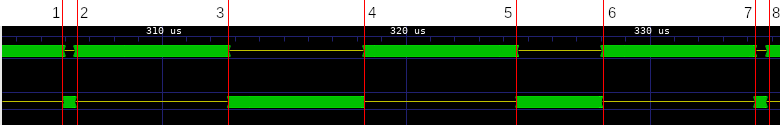
\includegraphics[width=1.\linewidth]{fb_perf}
  \caption{Performanse frame\_buffer modula}
  \label{fb_perf}
\end{figure}

Na gornjem interfejsu koji predstavlja izlaz ii\_gen modula može se videti
prvi period pauze negde oko 305 us.
Tada je generisanje integralne slike gotovo i klasifikator počinje sa radom.
U ovom slučaju trajanje rada klasifikatora je kratko zbog toga što je prozor
odbačen posle prve etape. \\

U narednoj periodu pauze gornjeg interfejsa negde oko 315 - 318 us može se
videti značajno duže vreme pauze.
Tada je klasifikator dostigao neku od viših etapa, pa je tek kasnije odbacio
prozor.
Može se videti da se u ovom periodu može izračunati ceo prozor integralne slike
tokom rada klasifikatora.
Kako bi se ovo odradilo potrebno je duplirati frame\_buffer memoriju.

\subsubsection{Paralelno računanje prve etape}

Kao što se vidi na grafiku(\ref{cascade_classifier_img2}) prva etapa će se
izvršiti u svakom analiziranom prozoru, izvršavanje svake naredne etape
eksponencijalno opada.
Posle 5. etape procenat izvršavanja je manje od 1\%.
Prva etapa ima 9 obeležja, a zatim svaka naredna
eksponencijalno više.
Pošto će se veliki procenat vremena prilikom rada IP jezgra provesti na
računanje prve etape, računanje ove etape bi se moglo računati posebnim
prilagođenim klasifikatorom.

\subsubsection{Paralelni klasifikatori}

Kako bi se omogućio rad paralelnih klasifikatora, potrebno je izdeliti ulaznu
IMG RAM memoriju na regione.
Tako da će svaki paralelni klasifikator obrađivati svoj region. \\

U ovom slučaju treba umnožiti ii\_gen, sii\_gen, frame\_buffer, stddev module.
Adresu za čitanje koju generiše rd\_addrgen je moguće izvesti za svaki region
uvođenjem offset-a adrese, tako da rd\_addrgen nije potrebno umnožiti u ovom
slučaju.
Moguće je koristiti jednu features\_mem memoriju za sve paralelne klasifikatore,
ali u tom slučaju svi paralelni klasifikatori će raditi brzinom najsporijeg
klasifikatora.
Moguće je ponovno koristiti i memorije iz classifier modula, što uvesti isti
efekat kao i features\_mem memorije.
Aritmetičke operatore iz classifier modula je potrebno umnožiti.

\subsubsection{Računanje više obeležja u paraleli}
Kao što se može videti na blok dijagramu klasifikatora(\ref{classifier_bd})
trenutno se jedno obeležje računa u trenutku.
Potrebno je četiri takta da se površina jednog pravougaonika izračuna.
Moguće je računati 2 obeležja u paraleli.
U tom slučaju bi frame\_buffer memorija bila duplirana zbog većeg broja portova
za čitanje.
Dok bi features\_mem memorija bila značajno komplikovanija, kao i classifier modul.

\subsubsection{Računanje skaliranih slika u paraleli}

Kao što se može videti na slici(\ref{image_pyramid}) originalna slika se mora
obrađivati više puta nakon skaliranja.
Rezultati obrade slika na različitim skalama nemaju međusobnu zavisnost, zbog
toga je moguće obrađivati ih u paraleli. \\

Primenom ove optimizacije ne može se dobiti linearno uvećanje brzine.
Pošto je najviše vremena potrebno da se obradi originalna slika, dok je za svaku
narednu skaliranu sliku potrebno sve manje vremena za obradu.
Dobitak performansi ove optimizacije verovatno nije opravdan za dodatne
hardverske resurse.


\newpage
\section{Zaključak}

U ovom radu je uspešno projektovana arhitektura hardverskog akceleratora
Viola-Jones algoritma.
Performanse hardverskog rešenja nisu dostigle performanse OpenCV softverske
implementacije. \\

Predloženim optimizacijama moguće je dostići približne performanse OpenCV
implementacije.
Bolje performanse bi se postigle i korišćenjem većeg i kvalitetnijeg FPGA čipa,
na kojem bi se sistem implementirao sa višom frekvencijom takta.
U slučaju \gls{asic} implementacije moguće je dostići mnogo više
frekvencije rada, pa dobiti značajno brže rešenje od softverskog. \\

Tokom implementacije hardverske arhitekture korišćen je inovativni pristup opisa
hardvera korišćenjem PyGears metodologije.
Takođe ista arhitektura je implementirana i u standardnoj RTL SystemVerilog
implementaciji.
Zaključeno je da funkcionalni pristup koji nameće PyGears metodologija može
značajno ubrzati razvoj u nekim situacijama, dok je pojedine komponente
jednostavnije implementirati RTL metodologijom. \\
Dodatni hardverski resursi u slučaju PyGears metodologije mogu biti zanemarljivi
za manje dizajnove i FPGA čipove.
U slučaju ASIC implementacije često je potrebno dobiti minimalnu implementaciju i
tada dodatni hardverski resursi uveliko utiču na cenu i performanse, u tom
slučaju RTL metodologija ima veliku prednost. \\

U radu je uspešno implementiran sistem na Zynq SoC platformi, prilikom
čega je bilo potrebno napisati Linux Device Driver.
Isto tako i konfigurisati i kompajlirati U-Boot i Linux Kernel za potrebe
projektovanog embeded sistema. \\
Napisana korisnička aplikacija u dva hijerarhijska nivoa, omogućava jednostavnu
komunikaciju sa projektovanim Kernel Driver-om iz različitih programskih jezika.
U ovom slučaju najviši nivo hijerarhije korisničke aplikacije je napisan u
Python-u. \\

\newpage

\bibliography{bibliography}
\bibliographystyle{IEEEtran}

\end{document}

% Local Variables:
% TeX-command-extra-options: "-shell-escape"
% End: